\documentclass[tikz,border=10pt]{standalone}
\usepackage[T1]{fontenc}
\usepackage[utf8]{inputenc}
\usepackage{tikz}
\usetikzlibrary{arrows.meta, positioning, calc, fit, backgrounds, shapes.geometric}

% ── Thesis palette anchored to engineering red rgb(0.549,0.176,0.098) ──
% Red family (parse failure / correction path)
\definecolor{redFill}{HTML}{F5E8E4}
\definecolor{redLine}{HTML}{8C2D18}
\definecolor{redText}{HTML}{3A1009}
% Slate family (model generation)
\definecolor{slateFill}{HTML}{EAEDF0}
\definecolor{slateLine}{HTML}{6B7E8C}
\definecolor{slateText}{HTML}{2E404D}
% Sand family (terminal / exhausted)
\definecolor{sandFill}{HTML}{FAF5EE}
\definecolor{sandLine}{HTML}{B8A070}
\definecolor{sandText}{HTML}{5A4118}
% Teal family (commit / positive outcome)
\definecolor{tealFill}{HTML}{E5F0ED}
\definecolor{tealLine}{HTML}{3D7A6A}
\definecolor{tealText}{HTML}{1E4D41}
% Neutrals
\definecolor{arrowGray}{HTML}{8A8880}
\definecolor{phaseText}{HTML}{3D3C38}

\begin{document}
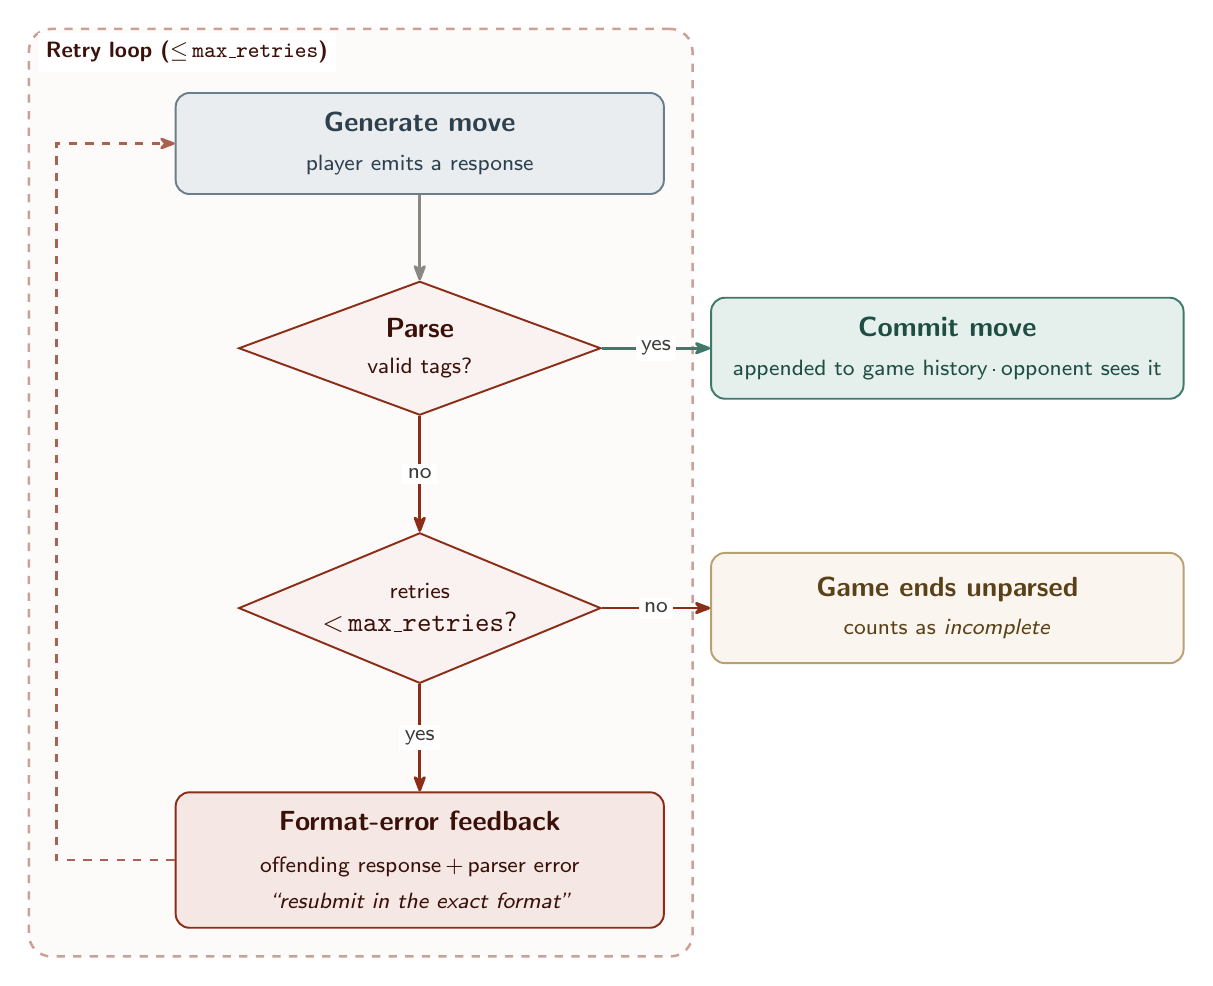
\begin{tikzpicture}[
  font=\sffamily,
  box/.style    ={rounded corners=5pt, draw, line width=0.7pt, align=center, inner sep=7pt},
  gen/.style    ={box, fill=slateFill, draw=slateLine, text=slateText,
                  minimum width=6.2cm, minimum height=1.15cm},
  feedback/.style={box, fill=redFill,  draw=redLine,   text=redText,
                  minimum width=6.2cm, minimum height=1.7cm},
  commit/.style ={box, fill=tealFill,  draw=tealLine,  text=tealText,
                  minimum width=6.0cm, minimum height=1.15cm},
  terminal/.style={box, fill=sandFill, draw=sandLine,  text=sandText,
                  minimum width=6.0cm, minimum height=1.4cm},
  dec/.style    ={diamond, aspect=2.1, draw=redLine, fill=redFill!55, text=redText,
                  line width=0.7pt, align=center, inner sep=1pt,
                  minimum width=4.6cm, minimum height=1.7cm},
  edgelbl/.style={font=\sffamily\footnotesize, text=phaseText, fill=white, inner sep=2pt},
  flow/.style   ={-{Stealth[round]}, draw=arrowGray, line width=1pt},
  good/.style   ={-{Stealth[round]}, draw=tealLine,  line width=1pt},
  bad/.style    ={-{Stealth[round]}, draw=redLine,   line width=1pt},
  back/.style   ={-{Stealth[round]}, draw=redLine!75, line width=0.9pt, dashed},
]

% ----- Main vertical spine -----
\node[gen] (GEN) at (0, 0)
  {\textbf{Generate move}\\[2pt]
   \footnotesize player emits a response};

\node[dec] (PARSE) at (0, -2.6)
  {\textbf{Parse}\\[1pt]\footnotesize valid tags?};

\node[dec] (BUDGET) at (0, -5.9)
  {\footnotesize retries\\$<$\,\texttt{max\_retries}?};

\node[feedback] (FB) at (0, -9.1)
  {\textbf{Format-error feedback}\\[3pt]
   \footnotesize offending response\,+\,parser error\\[1pt]
   \footnotesize \emph{``resubmit in the exact format''}};

% ----- Right column: success / exhausted -----
\node[commit] (COMMIT) at (6.7, -2.6)
  {\textbf{Commit move}\\[2pt]
   \footnotesize appended to game history\,·\,opponent sees it};

\node[terminal] (END) at (6.7, -5.9)
  {\textbf{Game ends unparsed}\\[2pt]
   \footnotesize counts as \emph{incomplete}};

% ----- Arrows on the spine -----
\draw[flow] (GEN.south) -- (PARSE.north);
\draw[bad]  (PARSE.south) -- node[edgelbl, pos=0.5] {no} (BUDGET.north);
\draw[bad]  (BUDGET.south) -- node[edgelbl, pos=0.5] {yes} (FB.north);

% ----- Success / exhausted branches -----
\draw[good] (PARSE.east) -- node[edgelbl, pos=0.5] {yes} (COMMIT.west);
\draw[bad]  (BUDGET.east) -- node[edgelbl, pos=0.5] {no} (END.west);

% ----- Loop-back: feedback regenerates the move -----
\coordinate (fbLeft)  at ($(FB.west)  + (-1.5,0)$);
\coordinate (genLeft) at ($(GEN.west) + (-1.5,0)$);
\draw[back] (FB.west) -- (fbLeft) -- (genLeft) -- (GEN.west);
\node[font=\sffamily\footnotesize, text=redText, anchor=east, rotate=90]
  at ($(fbLeft)!0.5!(genLeft) + (-0.05,0)$) {};

% ----- Dashed enclosure for the bounded retry loop -----
\coordinate (boxTop) at ($(GEN.north)+(0,0.45)$);
\begin{scope}[on background layer]
  \node[draw=redLine!45, dashed, rounded corners=8pt, line width=0.9pt,
        fit=(PARSE)(BUDGET)(FB)(genLeft)(boxTop), inner sep=10pt,
        fill=redFill!18] (LOOPBOX) {};
\end{scope}
\node[font=\sffamily\bfseries\footnotesize, text=redText, anchor=north west, fill=white, inner sep=3pt]
  at ($(LOOPBOX.north west)+(0.12,-0.06)$) {Retry loop ($\le$\,\texttt{max\_retries})};

\end{tikzpicture}
\end{document}
